%%%%%%%%%%%%%%%%%%%%%%%%%%%%%%%%%%%%%%%%%%%%%%%%%%%%%%%%%%%%
%%  This Beamer template was created by Cameron Bracken.
%%  Anyone can freely use or modify it for any purpose
%%  without attribution.
%%
%%  Last Modified: January 9, 2009
%%

\documentclass[xcolor=x11names,compress]{beamer}

%% General document %%%%%%%%%%%%%%%%%%%%%%%%%%%%%%%%%%
\usepackage{graphicx}
%%%%%%%%%%%%%%%%%%%%%%%%%%%%%%%%%%%%%%%%%%%%%%%%%%%%%%

\usepackage[frenchb]{babel}

\usepackage[utf8]{inputenc}

\usepackage{lastpage}

\usepackage[numbers]{natbib} \newcommand{\newblock}{}

\usepackage{caption}
\captionsetup{figurename=}

\usepackage{pgffor}

%% Beamer Layout %%%%%%%%%%%%%%%%%%%%%%%%%%%%%%%%%%
\useoutertheme[subsection=false,shadow]{miniframes}
\useinnertheme{default} \usefonttheme{serif} \usepackage{palatino}

\setbeamerfont{title like}{shape=\scshape}
\setbeamerfont{frametitle}{shape=\scshape}
\setbeamerfont{footline}{shape=\scshape}

\setbeamercolor*{lower separation line head}{bg=DeepSkyBlue4}
\setbeamercolor*{normal text}{fg=black,bg=white}
\setbeamercolor*{alerted text}{fg=red} \setbeamercolor*{example
  text}{fg=black} \setbeamercolor*{structure}{fg=black}

\setbeamercolor*{palette tertiary}{fg=black,bg=black!10}
\setbeamercolor*{palette quaternary}{fg=black,bg=black!10}

\setbeamercolor{footlinerule}{bg=DeepSkyBlue4}
\setbeamercolor*{footlinecolor}{bg=black!10}

\renewcommand{\(}{\begin{columns}} \renewcommand{\)}{\end{columns}}
\newcommand{\<}[1]{\begin{column}{#1}} \renewcommand{\>}{\end{column}}
%%%%%%%%%%%%%%%%%%%%%%%%%%%%%%%%%%%%%%%%%%%%%%%%%%


\author{Arnaud Bletterer - UDS} \title{Outils multidimensionnels de
  déformation}

\newcommand\mytext{Outils multidimensionnels de déformation}

\graphicspath{{PresentationFigs/}}

\makeatother \setbeamertemplate{footline} {%
  \leavevmode
  \begin{beamercolorbox}[wd=\paperwidth,ht=1ex,dp=0ex,center]{footlinerule}
  \end{beamercolorbox}%

  \hbox{\begin{beamercolorbox}[wd=1\paperwidth,ht=2.5ex,dp=1.125ex,leftskip=.3cm,rightskip=.3cm]{footlinecolor}%
      \count1 = \inserttotalframenumber
      \count3 = \paperwidth
      \divide\count3 by \count1

      \foreach \n in
      {\insertpagenumber,...,\count1}{\hskip \count1 px}
      
\includegraphics[scale=0.05, viewport=0 65 0 0]{alligator-ouvert}
   
    \end{beamercolorbox}
  }

  \hbox{\begin{beamercolorbox}[wd=.5\paperwidth,ht=2.5ex,dp=1.125ex,leftskip=.3cm,rightskip=.3cm]{footlinecolor}%
      \inserttitle
    \end{beamercolorbox}%

    \begin{beamercolorbox}[wd=.5\paperwidth,ht=2.5ex,dp=1.125ex,leftskip=.3cm,rightskip=.3cm]{footlinecolor}%
      \usebeamerfont{author in head/foot}\insertauthor\hfill
      \insertpagenumber /\inserttotalframenumber
    \end{beamercolorbox}}%
  \vskip0pt%
} \makeatletter

\begin{document}

%%%%%%%%%%%%%%%%%%%%%%%%%%%%%%%%%%%%%%%%%%%%%%%%%%%%%%
%%%%%%%%%%%%%%%%%%%%%%%%%%%%%%%%%%%%%%%%%%%%%%%%%%%%%%
\section{\scshape Introduction}
\begin{frame}
  \title{Outils multidimensionnels de déformation\\~\\

    \begin{figure}
      \begin{center}
      
\includegraphics[scale=0.3]{uds-logo}~~~~~~~~~
      
\includegraphics[scale=0.15]{icube-logo}
      \end{center}
    \end{figure}
  } \date{\vspace{0.5cm} \today }

  \author{Arnaud Bletterer\\
    \it Université de Strasbourg}

  \titlepage
\end{frame}

%%%%%%%%%%%%%%%%%%%%%%%%%%%%%%%%%%%%%%%%%%%%%%%%%%%%%%
%%%%%%%%%%%%%%%%%%%%%%%%%%%%%%%%%%%%%%%%%%%%%%%%%%%%%%
\begin{frame}{Sommaire}
  \tableofcontents
\end{frame}

%%%%%%%%%%%%%%%%%%%%%%%%%%%%%%%%%%%%%%%%%%%%%%%%%%%%%%
%%%%%%%%%%%%%%%%%%%%%%%%%%%%%%%%%%%%%%%%%%%%%%%%%%%%%%
\section{\scshape Etat de l'art}
\subsection{Introduction}
\begin{frame}{}
  \begin{figure}[h]
    \begin{center}
      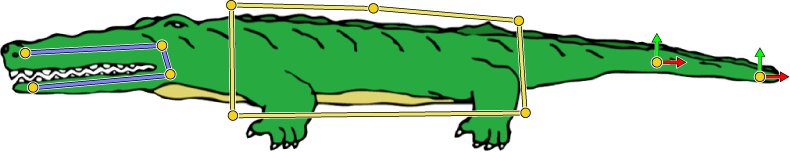
\includegraphics[scale=0.2]{alligator-avant.png}
      
\includegraphics[scale=0.2]{alligator-apres.png}
    \end{center}
\caption{Image de \citet{JBPS11}}
  \end{figure}
  \begin{itemize}
  \item Item A
  \item Item B
    \begin{itemize}
    \item Subitem 1
    \item Subtem 2
    \end{itemize}
  \item Item C
  \end{itemize}
\end{frame}


%%%%%%%%%%%%%%%%%%%%%%%%%%%%%%%%%%%%%%%%%%%%%%%%%%%%%%
%%%%%%%%%%%%%%%%%%%%%%%%%%%%%%%%%%%%%%%%%%%%%%%%%%%%%%
\section{\scshape Méthode implémentée}
\subsection{frame}
\begin{frame}{frame}

\end{frame}

%%%%%%%%%%%%%%%%%%%%%%%%%%%%%%%%%%%%%%%%%%%%%%%%%%%%%%
%%%%%%%%%%%%%%%%%%%%%%%%%%%%%%%%%%%%%%%%%%%%%%%%%%%%%%
\section{\scshape Continuité}
\begin{frame}{Continuité}

\end{frame}

\begin{frame}{References}

\bibliography{../Rapport/References/references.bib}

\end{frame}


\end{document}